% Schwarzschild Coordinates Comparison
% File: tikz_schwarzschild_coordinates.tex
% Purpose: Visualize multiple coordinate systems on same spacetime geometry
% For: Chapter 1 - Mathematical Preliminaries

\begin{figure}[htbp]
\centering
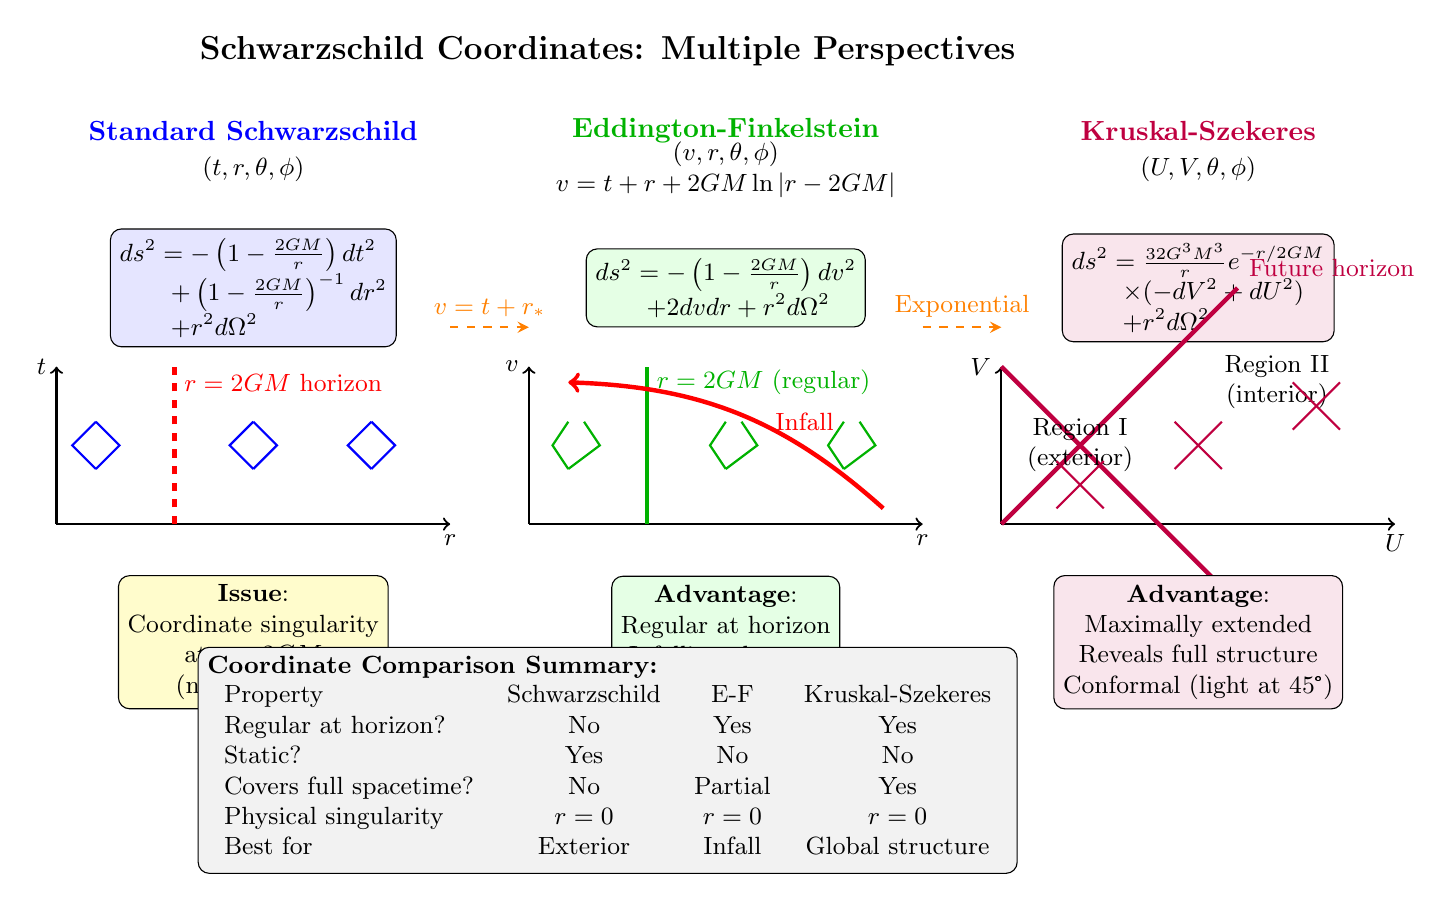
\begin{tikzpicture}[scale=1.0, every node/.style={font=\small}]

% Title
\node[font=\bfseries\large] at (7, 5.5) {Schwarzschild Coordinates: Multiple Perspectives};

% Left panel: Standard Schwarzschild (t, r, theta, phi)
\begin{scope}[shift={(0,0)}]
    \node[font=\bfseries, blue] at (2.5, 4.5) {Standard Schwarzschild};
    \node[align=center] at (2.5, 4) {$(t, r, \theta, \phi)$};
    
    % Metric
    \node[draw, fill=blue!10, align=left, rounded corners] at (2.5, 2.5) {
        $ds^2 = -\left(1-\frac{2GM}{r}\right)dt^2$\\
        \qquad $+ \left(1-\frac{2GM}{r}\right)^{-1}dr^2$\\
        \qquad $+ r^2 d\Omega^2$
    };
    
    % Spacetime diagram
    \draw[thick, ->] (0, -0.5) -- (0, 1.5) node[left] {$t$};
    \draw[thick, ->] (0, -0.5) -- (5, -0.5) node[below] {$r$};
    
    % Event horizon
    \draw[red, ultra thick, dashed] (1.5, -0.5) -- (1.5, 1.5);
    \node[red, right] at (1.5, 1.3) {$r=2GM$ horizon};
    
    % Light cones
    \foreach \x in {0.5, 2.5, 4} {
        \draw[blue, thick] (\x, 0.2) -- (\x+0.3, 0.5) -- (\x, 0.8);
        \draw[blue, thick] (\x, 0.2) -- (\x-0.3, 0.5) -- (\x, 0.8);
    }
    
    % Issue annotation
    \node[draw, fill=yellow!20, align=center, rounded corners] at (2.5, -2) {
        \textbf{Issue}:\\
        Coordinate singularity\\
        at $r=2GM$\\
        (not physical)
    };
\end{scope}

% Middle panel: Eddington-Finkelstein (v, r, theta, phi)
\begin{scope}[shift={(6,0)}]
    \node[font=\bfseries, green!70!black] at (2.5, 4.5) {Eddington-Finkelstein};
    \node[align=center] at (2.5, 4) {$(v, r, \theta, \phi)$\\$v = t + r + 2GM\ln|r-2GM|$};
    
    % Metric
    \node[draw, fill=green!10, align=left, rounded corners] at (2.5, 2.5) {
        $ds^2 = -\left(1-\frac{2GM}{r}\right)dv^2$\\
        \qquad $+ 2dvdr + r^2 d\Omega^2$
    };
    
    % Spacetime diagram
    \draw[thick, ->] (0, -0.5) -- (0, 1.5) node[left] {$v$};
    \draw[thick, ->] (0, -0.5) -- (5, -0.5) node[below] {$r$};
    
    % Event horizon (regular now)
    \draw[green!70!black, ultra thick] (1.5, -0.5) -- (1.5, 1.5);
    \node[green!70!black, right] at (1.5, 1.3) {$r=2GM$ (regular)};
    
    % Light cones (tilted inward)
    \foreach \x in {0.5, 2.5, 4} {
        \draw[green!70!black, thick] (\x, 0.2) -- (\x+0.4, 0.5) -- (\x+0.2, 0.8);
        \draw[green!70!black, thick] (\x, 0.2) -- (\x-0.2, 0.5) -- (\x, 0.8);
    }
    
    % Infalling path
    \draw[red, ultra thick, ->] (4.5, -0.3) to[bend right=20] (0.5, 1.3);
    \node[red] at (3.5, 0.8) {Infall};
    
    % Advantage annotation
    \node[draw, fill=green!10, align=center, rounded corners] at (2.5, -2) {
        \textbf{Advantage}:\\
        Regular at horizon\\
        Infalling observer\\
        perspective
    };
\end{scope}

% Right panel: Kruskal-Szekeres (U, V, theta, phi)
\begin{scope}[shift={(12,0)}]
    \node[font=\bfseries, purple] at (2.5, 4.5) {Kruskal-Szekeres};
    \node[align=center] at (2.5, 4) {$(U, V, \theta, \phi)$};
    
    % Metric
    \node[draw, fill=purple!10, align=left, rounded corners] at (2.5, 2.5) {
        $ds^2 = \frac{32G^3M^3}{r}e^{-r/2GM}$\\
        \qquad $\times (-dV^2 + dU^2)$\\
        \qquad $+ r^2 d\Omega^2$
    };
    
    % Spacetime diagram (conformal)
    \draw[thick, ->] (0, -0.5) -- (0, 1.5) node[left] {$V$};
    \draw[thick, ->] (0, -0.5) -- (5, -0.5) node[below] {$U$};
    
    % Horizons (45 degree lines)
    \draw[purple, ultra thick] (0, -0.5) -- (3, 2.5) node[above right] {Future horizon};
    \draw[purple, ultra thick] (0, 1.5) -- (3, -1.5);
    
    % Regions
    \node[align=center] at (1, 0.5) {Region I\\(exterior)};
    \node[align=center] at (3.5, 1.3) {Region II\\(interior)};
    
    % Light cones (45 degrees everywhere)
    \foreach \x/\y in {1/0, 2.5/0.5, 4/1} {
        \draw[purple, thick] (\x, \y) -- (\x+0.3, \y+0.3);
        \draw[purple, thick] (\x, \y) -- (\x-0.3, \y+0.3);
        \draw[purple, thick] (\x, \y) -- (\x+0.3, \y-0.3);
        \draw[purple, thick] (\x, \y) -- (\x-0.3, \y-0.3);
    }
    
    % Advantage annotation
    \node[draw, fill=purple!10, align=center, rounded corners] at (2.5, -2) {
        \textbf{Advantage}:\\
        Maximally extended\\
        Reveals full structure\\
        Conformal (light at 45°)
    };
\end{scope}

% Comparison table at bottom
\node[draw, fill=gray!10, align=left, rounded corners] at (7, -3.5) {
    \textbf{Coordinate Comparison Summary:}\\
    \begin{tabular}{lccc}
    \toprule
    Property & Schwarzschild & E-F & Kruskal-Szekeres \\
    \midrule
    Regular at horizon? & No & Yes & Yes \\
    Static? & Yes & No & No \\
    Covers full spacetime? & No & Partial & Yes \\
    Physical singularity & $r=0$ & $r=0$ & $r=0$ \\
    Best for & Exterior & Infall & Global structure \\
    \bottomrule
    \end{tabular}
};

% Transformation arrows
\draw[->, >=stealth, thick, dashed, orange] (5, 2) -- (6, 2) node[midway, above] {$v=t+r_*$};
\draw[->, >=stealth, thick, dashed, orange] (11, 2) -- (12, 2) node[midway, above] {Exponential};

\end{tikzpicture}
\caption{Three coordinate systems for Schwarzschild spacetime. Standard Schwarzschild coordinates have coordinate singularity at event horizon. Eddington-Finkelstein coordinates regular at horizon, good for infalling observers. Kruskal-Szekeres coordinates maximally extended, reveal complete spacetime structure including black/white hole regions. All describe same physical geometry; coordinate choice determines what features are manifest. Table compares key properties.}
\label{fig:schwarzschild_coordinates}
\end{figure}
